%%%%%%%%%%%%%%%%%%%%%%%%%%%%%%%%%%%%%%%%%
% Journal Article
% LaTeX Template
% Version 1.3 (9/9/13)
%
% This template has been downloaded from:
% http://www.LaTeXTemplates.com
%
% Original author:
% Frits Wenneker (http://www.howtotex.com)
%
% License:
% CC BY-NC-SA 3.0 (http://creativecommons.org/licenses/by-nc-sa/3.0/)
%
%%%%%%%%%%%%%%%%%%%%%%%%%%%%%%%%%%%%%%%%%

%----------------------------------------------------------------------------------------
%	PACKAGES AND OTHER DOCUMENT CONFIGURATIONS
%----------------------------------------------------------------------------------------

\documentclass{article}

%\documentclass{aastex}  % version 5.0 or prior
%\usepackage{natbib}



\usepackage{graphicx}
\usepackage{lipsum} % Package to generate dummy text throughout this template
%\usepackage[sc]{mathpazo} % Use the Palatino font
\usepackage[T1]{fontenc} % Use 8-bit encoding that has 256 glyphs
\linespread{1.05} % Line spacing - Palatino needs more space between lines
\usepackage{microtype} % Slightly tweak font spacing for aesthetics

\usepackage[margin=1in,columnsep=20pt]{geometry} % Document margins
\usepackage{multicol} % Used for the two-column layout of the document
\usepackage[hang, small,labelfont=bf,up,textfont=it,up]{caption} % Custom captions under/above floats in tables or figures
\usepackage{booktabs} % Horizontal rules in tables
\usepackage{float} % Required for tables and figures in the multi-column environment - they need to be placed in specific locations with the [H] (e.g. \begin{table}[H])
\usepackage{hyperref} % For hyperlinks in the PDF
\usepackage{subcaption}

\usepackage{lettrine} % The lettrine is the first enlarged letter at the beginning of the text
\usepackage{paralist} % Used for the compactitem environment which makes bullet points with less space between them
\usepackage{amsmath}
\usepackage{abstract} % Allows abstract customization
\renewcommand{\abstractnamefont}{\normalfont\bfseries} % Set the "Abstract" text to bold
\renewcommand{\abstracttextfont}{\normalfont\small\itshape} % Set the abstract itself to small italic text

\usepackage{titlesec} % Allows customization of titles
%\renewcommand\thesection{\Roman{section}} % Roman numerals for the sections
%\renewcommand\thesubsection{\Roman{subsection}} % Roman numerals for subsections
%\renewcommand\thesubsubsection{\Alph{subsubsection}} % Roman numerals for subsections
\titleformat{\section}[block]{\LARGE\scshape}{\thesection}{1em}{} % Change the look of the section titles
\titleformat{\subsection}[block]{\Large\scshape}{\thesubsection}{1em}{} % Change the look of the section titles
\titleformat{\subsubsection}[block]{\large\scshape}{\thesubsubsection}{1em}{} % Change the look of the section titles

\usepackage{fancyhdr} % Headers and footers
\pagestyle{fancy} % All pages have headers and footers
\fancyhead{} % Blank out the default header
\fancyfoot{} % Blank out the default footer
\fancyhead[C]{Montana State University \quad $\bullet$ \quad CSCI 466 Artificial Intelligence \quad $\bullet$ \quad Group 21} % Custom header text
\fancyfoot[RO,LE]{\thepage} % Custom footer text

\newcommand{\ve}[1]{\boldsymbol{\mathbf{#1}}}

\title{\vspace{-15mm}\fontsize{24pt}{10pt}\selectfont\textbf{CSCI 446 Artificial Intelligence \\[2mm] Project 4 Final Report} } % Article title
\date{\today}
\author{
\large
\textsc{Roy Smart} \and \textsc{Nevin Leh} \and \textsc{Brian Marsh}\\[2mm] % Your name
}


%----------------------------------------------------------------------------------------

\begin{document}

	\maketitle % Insert title
	\thispagestyle{fancy} % All pages have headers and footers
	\normalsize

	\section{Introduction}
		Machine learning that is realized through an agent making actions and observing the results is known as reinforcement learning.  This type of learning is unsupervised, meaning that the “correct” solution given an input is not known from data.  Instead, the agent trains by observing many iterations of its own actions to maximize its cumulative rewards of its current problem.  For our project, we attempt to solve the racetrack problem by implementing reinforcement learning with the Value Iteration and Q-learning algorithms.
	\section{The Racetrack Problem}
		The racetrack problem involves controlling a car from start to finish along multiple given racetracks of varying size and shape.  Control is maintained solely by altering the velocity of the car.  The performance of the algorithm is scored by minimizing the number of time steps that the car takes in its run.  This can thus be improved by increasing velocity, but is also penalized if the car runs into a wall.  At any given state, the car is represented by the horizontal and vertical components of its location at time t, x(t) and y(t), respectively.  The velocity of the car is manipulated with the values of ax and ay.  Accompanying every acceleration action is a 20 percent chance of failure to create some variability for the agent.
	\section{Value Iteration}
	\subsection{Description}
	\textit{Value iteration} is a sequential reinforcement learning method for determining the optimal policy for a Markov decision process(MDP)\cite{Yu2013}. The algorithm calculates the utility for all of the states and then uses these utility values to determine the optimal action $a$ for each state $s$. To calculate utility we will be using the \textit{Bellman equation} as described in \cite{ai}. The equation is given as			
	\begin{equation}
	U(s) = R(s) + \gamma \max_{a \in A(s)}\sum_{s'} P(s'|s,a)U(s')
	\end{equation}
	where R(s) is the reward for the current state, $s'$ is the next state, and $P(s'|s,a)$ is the probability of being in state $s'$ given an action $a$ in state $s$. $\gamma$ is used to tweak how much weight we put on the expected next states utility values for calculating the current states utility value.
	
	Value iteration uses this equation to iteratively propagate utilities and actions to each state. To start each state is given a random utility, though each state still has a unique reward value with the goal states having high reward. We then iterate over every state, recalculating each states utility. We keep looping through the states until the largest change of utility, designated $\delta$, is larger than $\epsilon(1-\gamma)/\gamma$. $\epsilon$ designates the maximum error allowed in any state. This is a tunable value, with smaller numbers making convergence take longer.
	\subsection{Implementation}
	
	We based the design of our algorithm on the function \textsc{Value-Iteration} described in Figure 17.4 of \cite{ai}. 
	The table of utilities, computed using the \textit{Bellman equation}, was stored in a six-dimensional array representing every possible position, velocity and acceleration in both spatial dimensions.
	
	One addition we made during implementation was calculating the utility of each action for each possible velocity. This way, if a wall was hit, we would know what to do at a different velocity. This also helped combat the twenty percent chance that an action would fail.
	
	The two main tunable parameters are $\gamma$ and $\epsilon$. After doing some test runs, it was found that a smaller $\epsilon$ would generally have better results as seen in Table \ref{epsilon}. The results for $\gamma$ were not quite as clear. From Table \ref{gamma} it can be seen that a very high $\gamma$ seems to give better results. However, during further testing it was found that an extremely small $\epsilon$ counteracted this.
	\begin{table}
		\centering
		\begin{tabular}{|l|c|}
			\hline
			$\epsilon$ & Average Time \\ \hline
			1e-1 & 196.9 \\ 
			1e-3 & 18.1 \\
			1e-5 & 13.98\\
			1e-7 & 13.96 \\
			1e-9 & 14.12 \\ 
			1e-11 & 13.96 \\ \hline
		\end{tabular}
		\caption{Table of $\epsilon$ values and average times to complete the L-track. \\ The $\gamma$ value was set to 0.5 for all of the tests.}
		\label{epsilon}
	\end{table}
	
	\begin{table}
		\centering
		\begin{tabular}{|l|c|}
			\hline
			$\gamma$ & Average Time \\ \hline
			0.3 & 196.9 \\ 
			0.5 & 18.1 \\
			0.7 & 13.98\\
			0.9 & 13.96 \\ \hline
		\end{tabular}
		\caption{Table of $\gamma$ values and average times to complete the L-track.}
		\label{gamma}
	\end{table}
	\subsection{Experimental Design}
	
	\begin{table}
		\centering
		\begin{tabular}{|l|c|}
			\hline
			Parameter & Value \\ \hline
			Base Reward & 0.0 \\ 
			Wall Reward & 0.0 \\
			Finish Reward & 1.0 \\
			Discount Factor$(\gamma)$ & 0.5 \\
			Maximum Error$(\epsilon)$ & 1e-14 \\ \hline
		\end{tabular}
		\caption{Table of tunable values for the Value-iteration agent}
		\label{stuff}
	\end{table}
	The final values used in our experiment can be seen in Table \ref{stuff}. We chose a more moderate $\gamma$ of 0.5 since it showed better results with the extremely small $\epsilon$ we chose to do the experiment with. To find how well we did on each track we trained the algorithm on each track with the values above. After training, a single test run was done to find the time it took the algorithm to reach the finish line. 
	\section{$Q$-Learning}
		\subsection{Description}
			\textit{Q-learning} is a model-free reinforcement learning method for determining optimal action-selection policies \cite{ai}. An agent using this method leverages a quantity known as the $Q$-value to derive the optimal action $a$ for each state $s$. The $Q$-value, $Q(s,a)$ describes the expected utility for every action in every state within the environment and is learned by the agent using temporal difference learning.
			An expression to calculate the $Q$-value is given by \cite{ai} as
			\begin{equation}
				Q(s,a) \leftarrow Q(s,a) + \alpha \left[ R(s) + \gamma \max_{a'} Q(s',a') - Q(s,a) \right]
				\label{ql}
			\end{equation}
			where $a$ is the action that was executed in state $s$ that resulted in state $s'$ and $R(s)$ is the reward function. The constants $\alpha$ and $\gamma$ are known respectively as the learning rate and the discount factor. Equation \ref{ql} is used as an update rule to adjust the value of $Q(s,a)$ for each action-state pair in every time trial undertaken by the agent. Using this simple update rule and $Q$-values initialized to zero for every action-state, an agent can learn how to navigate an environment.
		\subsection{Implementation}
			We based the design of our algorithm on the function \textsc{Q-Learning-Agent} described in Figure 21.8 of \cite{ai}. 
			The table of action values, $Q[s,a]$ and the tabel of frequencies, $N[s,a]$ were stored in six-dimensional arrays representing every possible position, velocity and acceleration in both spatial dimensions.
			
			The agent took an astonishingly long time to train. To lower the training time, we adopted strategy where the agent was started close to the finish line and trained until convergence. The starting line was then moved back by $m$ squares and then again trained until convergence. This process was repeated until the actual start line had been reached. In this way, our $Q$-Learning agent could be incrementally trained, without having to wait around for a few months to complete training.
			
			To further improve training, we assigned a penalty to hitting the wall. We understand that this breaks the rules of the assignment slightly, but the training time was too preventative. This behavior could indicate a problem with our $Q$-Learning algorithm.
			
			The traditional way to detect convergence in $Q$-Learning is to measure the rate of change of the $Q$-values across the table, and exit once the rate is sufficiently small. We did not adopt this approach as it would have been computationally expensive. We instead opted for a convergence test based off of a running average of the timesteps required for $n$ trials.
			
			The learning rate, $\alpha$ and the discount factor, $\gamma$ were tuned by hand. The tuned parameters are outlined in Table \ref{Q_params};
			
			\begin{table}
				\centering
				\begin{tabular}{|l|c|}
					\hline
					Parameter & Value \\ \hline
					Base Reward & -1.0 \\ 
					Wall Reward & -2.0 \\
					Finish Reward & 1.0 \\
					Learning Rate & $1 \times 10^{-7}$ \\
					Discount Factor & 0.9 \\
					$m$ & 2 \\ \hline
				\end{tabular}
				\caption{Table of tunable values for the $Q$-Learning agent}
				\label{Q_params}
			\end{table}
		\subsection{Experimental Design}
		
			For our experiments, we measured the average number of time steps for the $Q$-Learning agent vs. the number of time trials. This has the effect of showing the rate of convergence of the $Q$-Learning algorithm and describing the overall performance of the algorithm as track complexity increases.
		
	\section{Results}		
				\begin{figure}[h!]
					\centering
					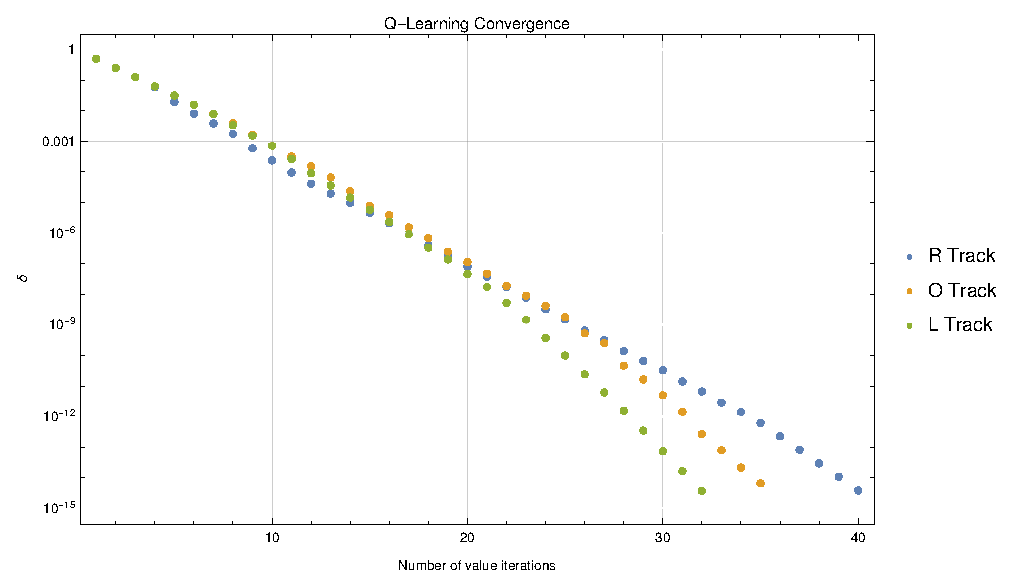
\includegraphics[width=0.8\textwidth]{Diagrams/VIter}
					\caption{}
					\label{VIter}
				\end{figure}
				
				The number of iterations to reach convergence for Value-Iteration was far smaller than for $Q$-Learning on all tracks as seen in figures \ref{VIter} and \ref{QLearn}. Consequently, the learning time was far shorter as well. It can also be seen that L-track took the least amount of iterations to converge out of all of the tracks. We theorize that this is the result of the track contained fewer curves and being generally shorter. The second fastest to converge was the O-track, and the third was the R-track. This seems to confirm our hypothesis because the R-track contained the most curves and was about the same size as the O-track.

				
				
				
				\begin{figure}[h!]
					\centering
					\includegraphics[width=\textwidth]{Diagrams/QLearn}
					\caption{}
					\label{QLearn}
				\end{figure}
				
				\begin{table}
					\centering
					\begin{tabular}{|l|c|c|}
						\hline
						Track & Algorithm & Time \\ \hline
						L-track & Value-Iteration & 22 \\ 
						L-track & $Q$-Learning & 23 \\ 
						O-track & Value-Iteration & 29 \\
						O-track & $Q$-Learning & 63 \\
						R-track & Value-Iteration & 33 \\
						R-track & $Q$-Learning & 63 \\
						R-track w/ restart & Value-Iteration & 139\\
						R-track w/ restart & $Q$-Learning & 221  \\ \hline
						
					\end{tabular}
					\caption{Table of results for Value-Iteration and $Q$-Learning on all three tracks. Each algorithm had one try to get to the finish.}
					\label{results}
				\end{table}
				
				Value-Iteration performed admirably in navigating the tracks as seen in Table \ref{results}. The algorithm was capable of navigating both the L-track and the O-track without hitting the walls on a semi regular basis. In addition, Value-Iteration outperformed Q-Learning on all of the tracks. As expected, the longer, curvier tracks took more time steps to finish. Finally, restarting the car at the start rather than at the last occupied square had drastic results on the time taken to finish the R-Track. It can be seen that the car still hits the wall regularly while navigating the tracks.


	\section{Conclusion}


	%\bibliographystyle{apj}
	\bibliographystyle{apalike}	
	\bibliography{sources}
\end{document}
